% Imported from algorithms/multimodal-position/README.md
\chapter{M04 多模态位置编码与媒体时钟}\label{seedance-m04}
\moduleinfo{M04}{基础方法与机制解释}{\hyperref[src-rope]{\texttt{rope}}、\hyperref[src-seedance-1.0]{\texttt{seedance-1.0}}、\hyperref[src-long-context-tuning]{\texttt{long-context-tuning}}、\hyperref[src-wan21-code]{\texttt{wan21-code}}、\hyperref[src-vincie-code]{\texttt{vincie-code}}}


Transformer 把输入组织成 token 序列，但一维排列顺序不足以描述视频结构。视觉 token 同时位于某个时间、某行和某列；文本 token 位于一句话中；多个镜头还各有自己的描述。多模态位置编码要保留这些不同的位置含义，让注意力知道内容之间的相对关系。

\section{RoPE 怎样把位置放进点积}\label{seedance-m04-rope-ux600eux6837ux628aux4f4dux7f6eux653eux8fdbux70b9ux79ef}

RoPE 将一对特征维度看成平面向量，按位置旋转。设旋转矩阵为：

\[
R(\phi)=\begin{bmatrix}
\cos\phi&-\sin\phi\\
\sin\phi&\cos\phi
\end{bmatrix}.
\]

位置为 \(m\) 的 query 和位置为 \(n\) 的 key，分别变为：

\[
q'_m=R(m\omega)q_m,\qquad k'_n=R(n\omega)k_n.
\]

由于旋转矩阵满足组合关系，点积可以写成：

\[
(q'_m)^\top k'_n=q_m^\top R((n-m)\omega)k_n.
\]

这样，显式引入的位置信息依赖相对距离 \(n-m\)。保持内容向量不变，同时把两个位置都平移 7，点积就保持不变。不过，网络中的内容向量本身已经受上下文影响，不能进一步推成``整个网络只依赖相对位置''。

不同特征对使用不同频率，常见形式为 \(\omega_i=b^{-2i/d_{\mathrm{rot}}}\)。旋转作用于投影后的 Q/K，位于注意力点积之前；V 通常不旋转，因为标准 RoPE 通过改变关注权重来引入位置。

\section{三维位置怎样进入同一个注意力头}\label{seedance-m04-ux4e09ux7ef4ux4f4dux7f6eux600eux6837ux8fdbux5165ux540cux4e00ux4e2aux6ce8ux610fux529bux5934}

注意力张量常写成 \codepath{B,h,N,d_h}：批大小、头数、token 数和单头维度。三维 RoPE 将最后的特征维度划给时间、高度、宽度三个轴，而不是复制三份 token。

\[
d_t+d_y+d_x\le d_h.
\]

每一段需要能成对旋转，通常取偶数；未参与旋转的通道可以原样保留。例如 \(d_h=12\)，三个轴各分 4 维。视觉 token 坐标为 \((t,y,x)\)，时间段使用 \(t\)，空间两段分别使用 \(y\) 和 \(x\)。

不同实现可能按相邻维配对，也可能将前后半段配对；配置中的数字也可能表示通道数或频率对数。迁移模型时，维度总和一致仍不足以证明布局兼容。

\section{多镜头怎样交错排列}\label{seedance-m04-ux591aux955cux5934ux600eux6837ux4ea4ux9519ux6392ux5217}

多镜头场景可以组织为``镜头描述、镜头视觉、下一镜头描述、下一镜头视觉''的交错序列。镜头内保留文本与视觉的位置关系，镜头之间再增加偏移。

\begin{figure}
\centering
\pandocbounded{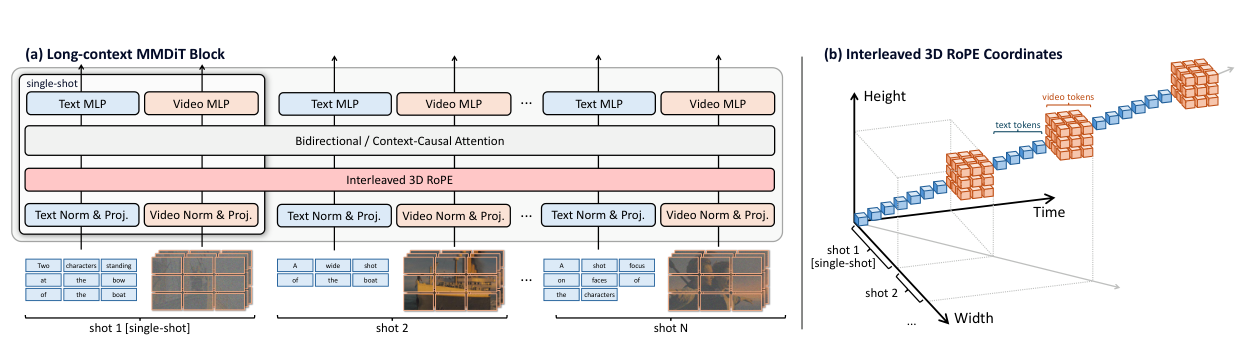
\includegraphics[keepaspectratio,alt={多镜头上下文与交错位置的组织 （论文示意，来源：long-context-tuning）}]{assets/seedance/figures/multishot-positions.png}}
\caption{多镜头上下文与交错位置的组织 （论文示意，来源：long-context-tuning）}
\end{figure}

图中左侧是跨镜头处理文本与视频的结构，右侧展示位置坐标如何随镜头追加。这种组织让相邻镜头具有不同的绝对位置，同时保留每个镜头内部原有的相对结构。

文本没有真实空间坐标，可以使用一维位置，或将同一个序列位置映射到多个轴。若频率和布局与原一维 RoPE 兼容，多轴形式可以退化为一维；若每轴重新起一组频率，则不一定与原实现完全相同。

\section{坐标、归属和可见性是三件事}\label{seedance-m04-ux5750ux6807ux5f52ux5c5eux548cux53efux89c1ux6027ux662fux4e09ux4ef6ux4e8b}

坐标回答``token 在哪里''；归属回答``这段描述或参考属于哪个镜头、哪个角色''；注意力掩码回答``哪些 token 允许互相读取''。三者需要一起设计。

例如，一张参考图只约束第二个镜头中的角色 A。即使为它设置了独立位置，也不能保证模型只把它用于角色 A。还需要角色和镜头绑定，必要时用显式 mask 限定可见范围。RoPE 只改变分数，并不会自动把不允许的连接设为负无穷。

同样，一组相同坐标既可以用于联合生成，也可以配合镜头间因果 mask 用于续写。因果性由信息流决定，不能仅凭坐标递增来判断。

\section{实现时最容易忽略的时间单位}\label{seedance-m04-ux5b9eux73b0ux65f6ux6700ux5bb9ux6613ux5ffdux7565ux7684ux65f6ux95f4ux5355ux4f4d}

视频帧号不是通用时间。固定 24 fps 的第 48 帧约对应两秒，可变帧率视频则需要读取实际时间戳；音频编码器可能每秒输出另一数量的 token。做音视频对齐时，应先把各模态位置映射到同一个物理时间轴，再决定编码方式。

检查一个位置编码实现，可以先验证坐标展平与还原是否一一对应，再检查 padding 是否被排除，最后测试同移坐标的点积性质。真正扩展到长视频时，还需要观察生成质量：位置编码能计算更远的坐标，不代表模型已经学会在这些坐标范围内保持角色、动作和剧情。

\section{从极简代码到真实实现}\label{seedance-m04-ux4eceux6781ux7b80ux4ee3ux7801ux5230ux771fux5b9eux5b9eux73b0}

对一对特征维度旋转时，真正改变的是 Q/K 的最后一维：

\begin{verbatim}
even, odd = x[..., 0::2], x[..., 1::2]
rotated_even = even * cos - odd * sin
rotated_odd = even * sin + odd * cos
\end{verbatim}

按三轴拆分再拼回的示例见 \hyperref[code-rope]{rope.py}。示例采用相邻维配对和各轴独立频率；真实 checkpoint 的布局应查 \href{https://github.com/Wan-Video/Wan2.1/blob/9737cba9c1c3c4d04b33fcad41c111989865d315/wan/modules/model.py}{Wan rope\_apply} 或 \href{https://github.com/ByteDance-Seed/VINCIE/blob/97cd2c5701e694dabcfea320c0cf59893d427fab/models/dit/rope.py}{VINCIE 多模态 RoPE}，不能仅看输出维数相同。
